\documentclass{article}
\usepackage[utf8]{inputenc}
\usepackage[T1]{fontenc}
\usepackage{graphicx}
\usepackage{float}
\begin{document}

\section*{Slide 1}

Radiation Studies on the

\begin{figure}[H]
\centering

\includegraphics[width=0.8\linewidth]{assets/Eduardo_IEEE_NSS_MIC_RTSD_Poster-2_slide_1_item_1.jpeg}
\end{figure}

ATLAS Link and Control Daughterboard

for the HL-LHC Upgrade

\begin{figure}[H]
\centering
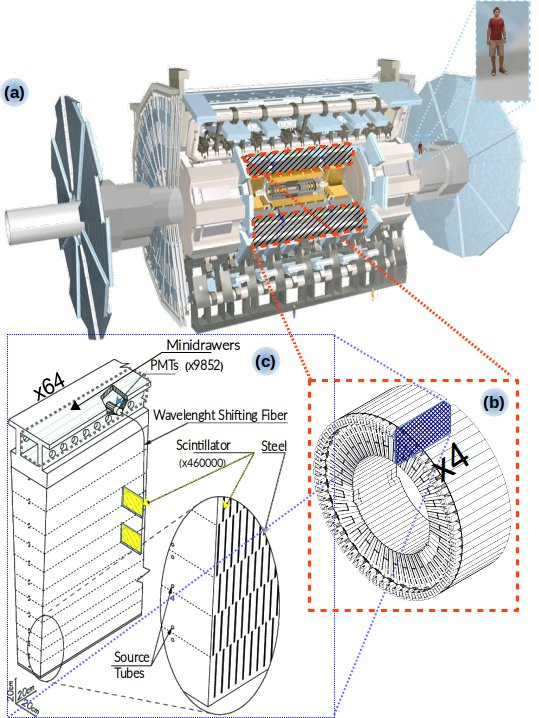
\includegraphics[width=0.8\linewidth]{assets/Eduardo_IEEE_NSS_MIC_RTSD_Poster-2_slide_1_item_2.jpeg}
\end{figure}

\begin{figure}[H]
\centering
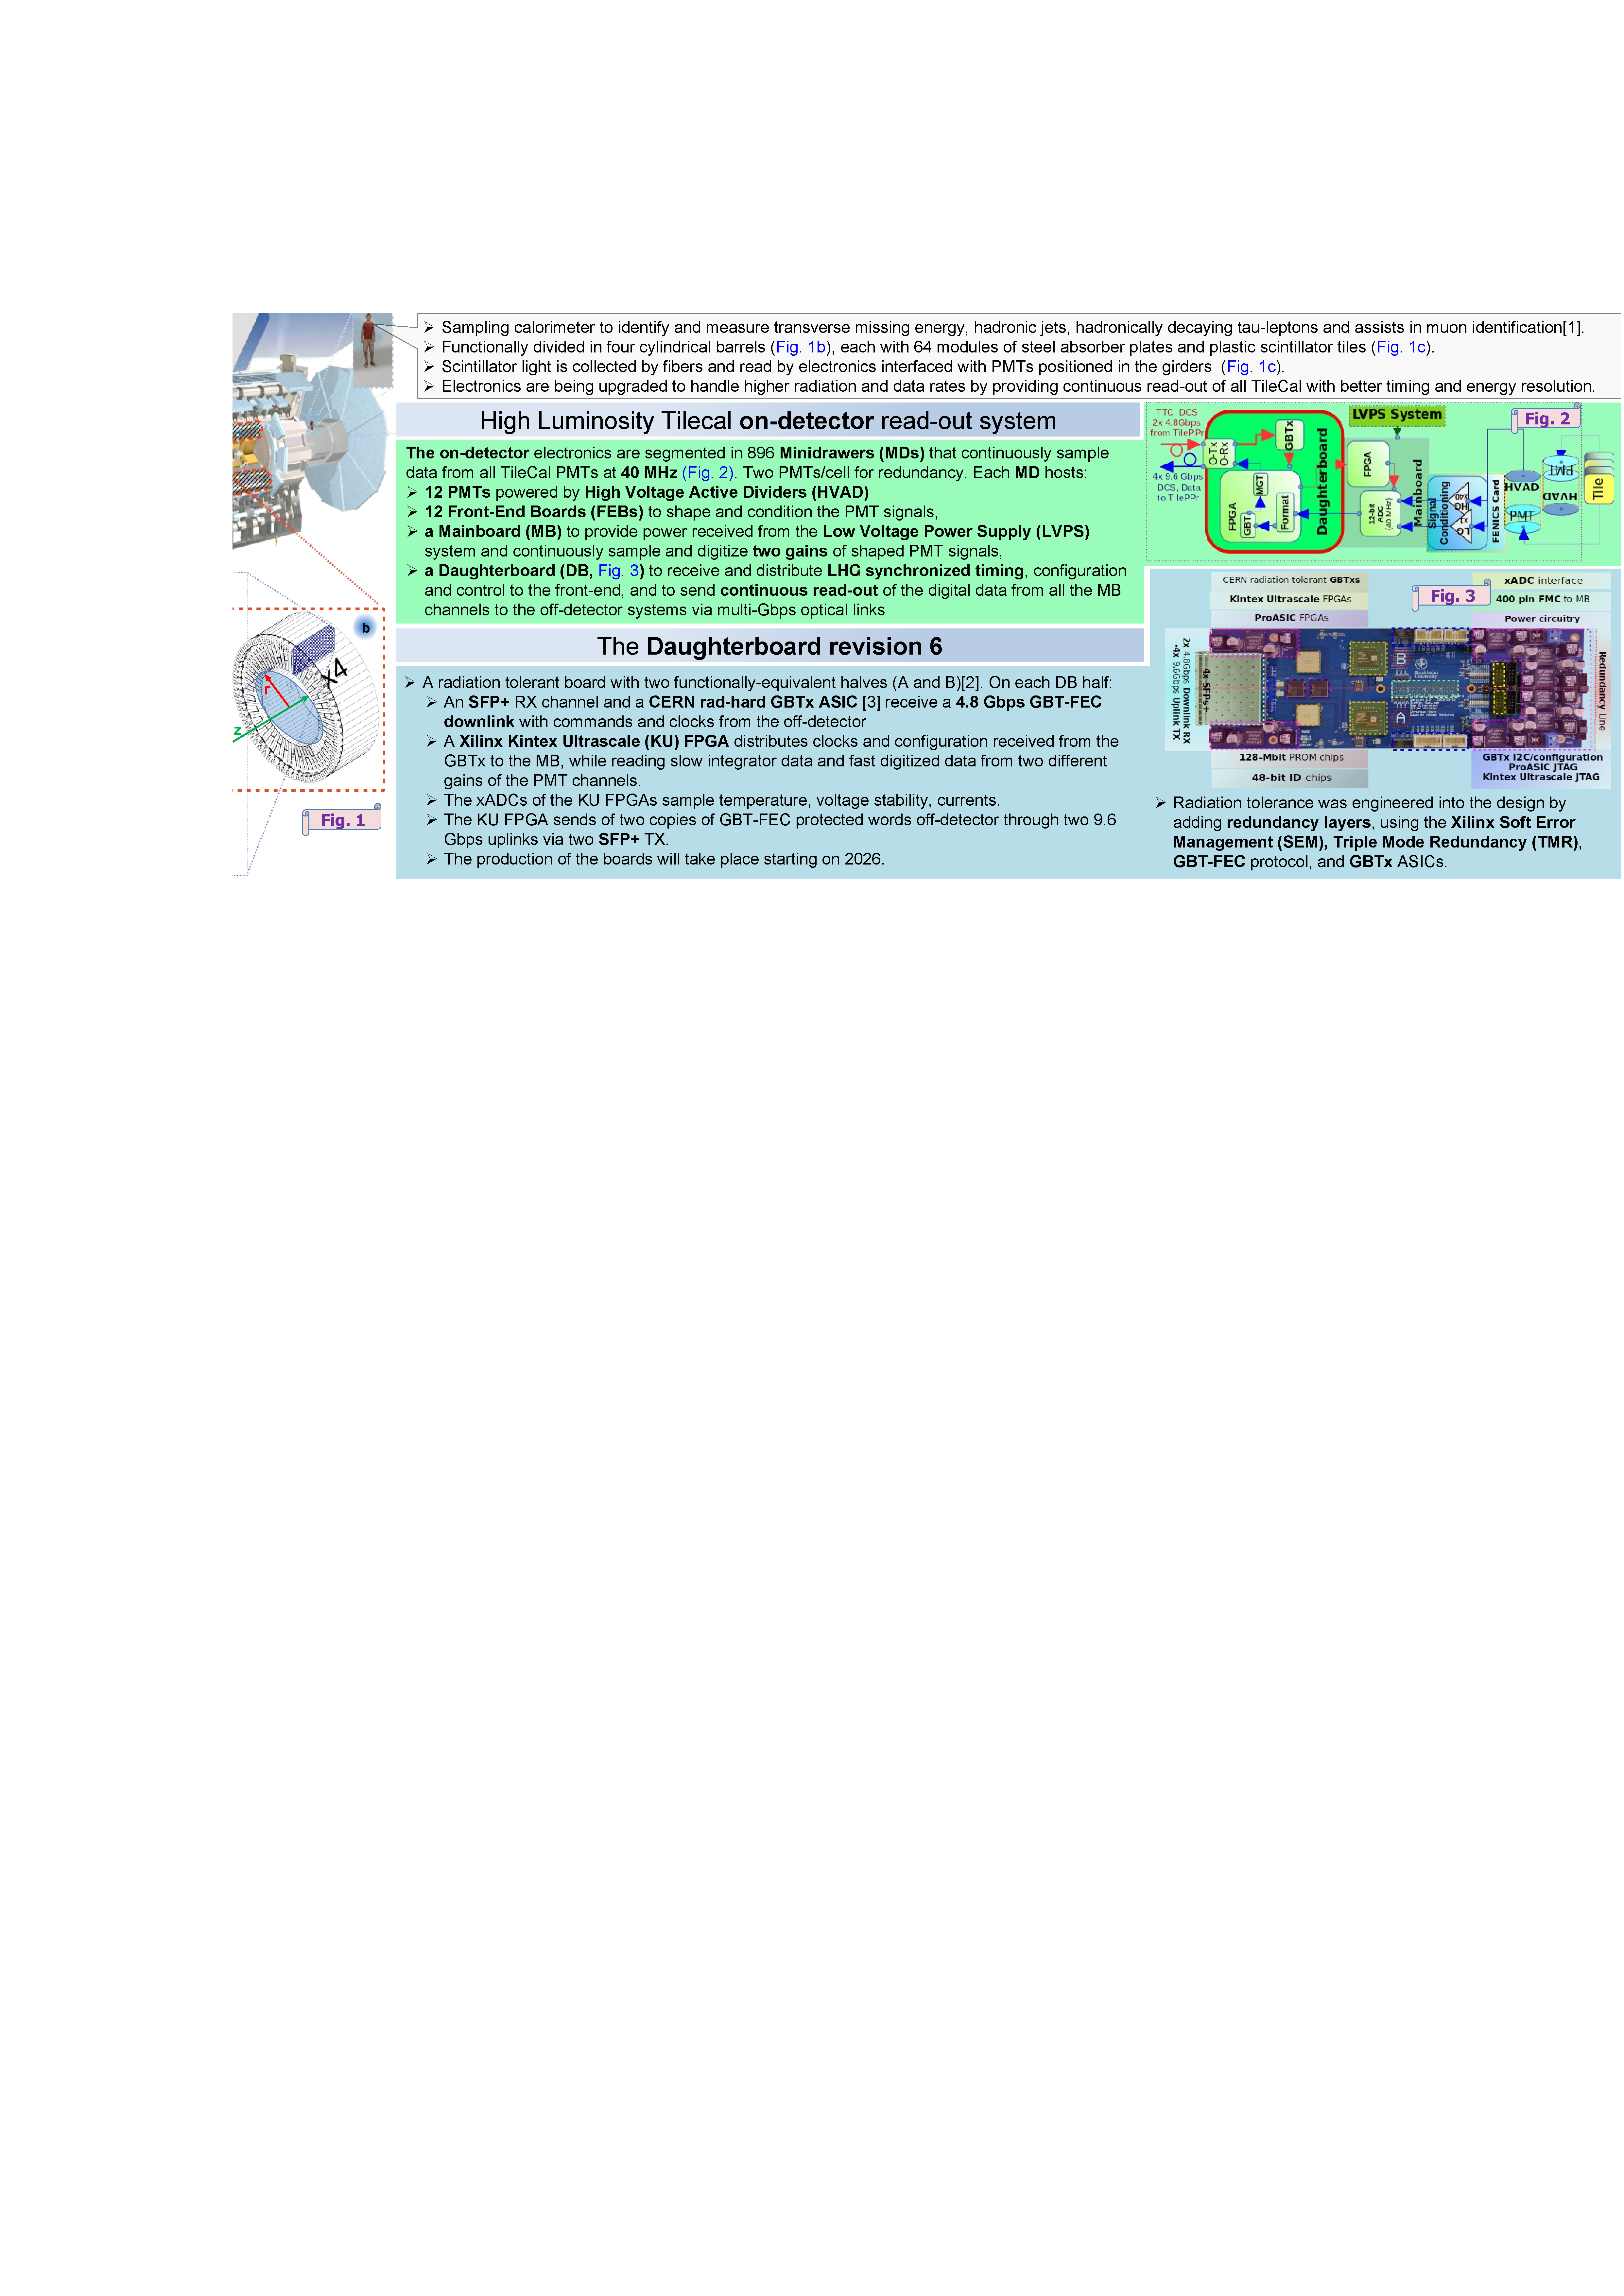
\includegraphics[width=0.8\linewidth]{assets/Eduardo_IEEE_NSS_MIC_RTSD_Poster-2_slide_1_item_3.pdf}
\end{figure}

a

\begin{figure}[H]
\centering
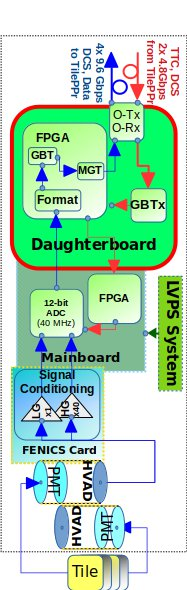
\includegraphics[width=0.8\linewidth]{assets/Eduardo_IEEE_NSS_MIC_RTSD_Poster-2_slide_1_item_4.jpeg}
\end{figure}

\begin{figure}[H]
\centering
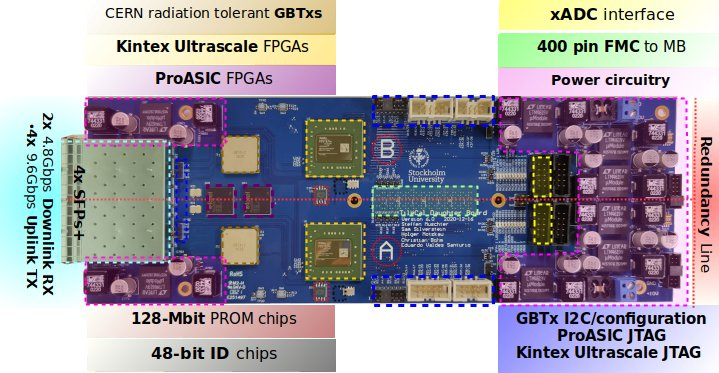
\includegraphics[width=0.8\linewidth]{assets/Eduardo_IEEE_NSS_MIC_RTSD_Poster-2_slide_1_item_5.jpeg}
\end{figure}

c

r

\begin{figure}[H]
\centering
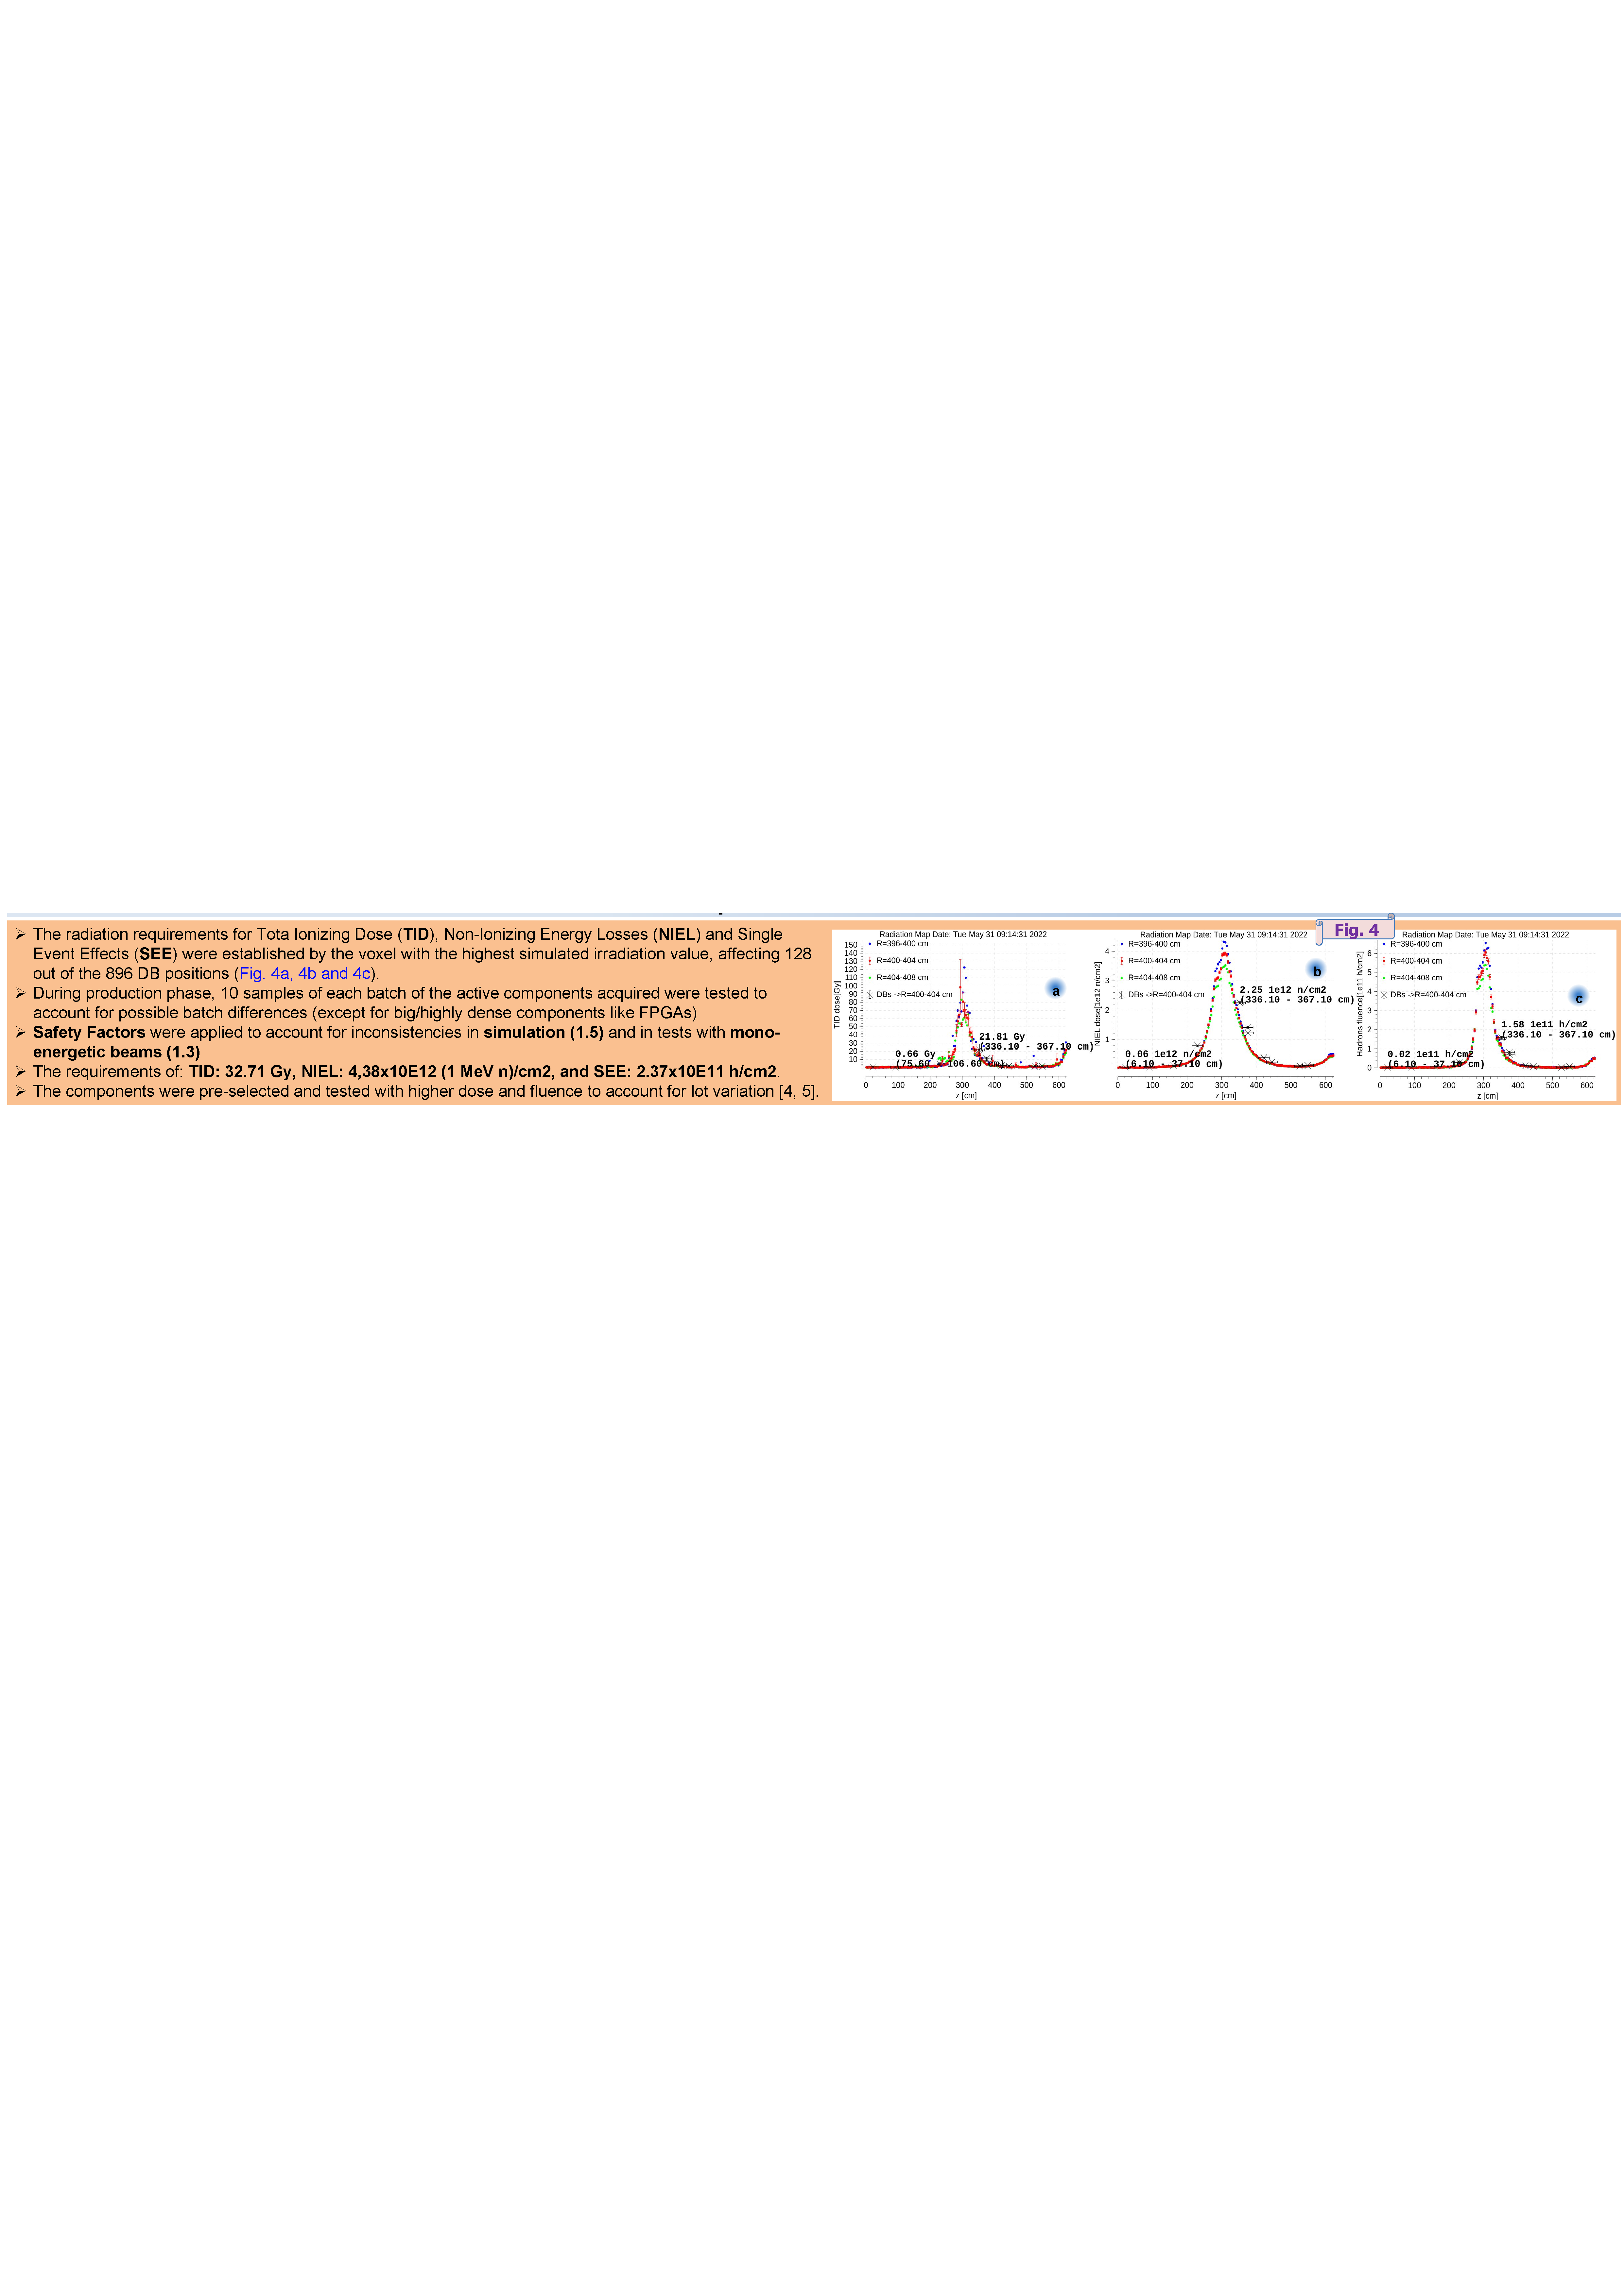
\includegraphics[width=0.8\linewidth]{assets/Eduardo_IEEE_NSS_MIC_RTSD_Poster-2_slide_1_item_6.pdf}
\end{figure}

\begin{figure}[H]
\centering
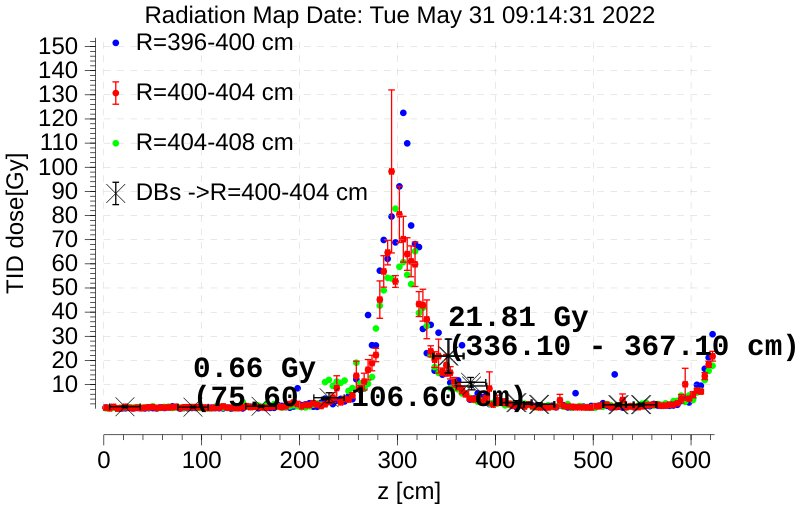
\includegraphics[width=0.8\linewidth]{assets/Eduardo_IEEE_NSS_MIC_RTSD_Poster-2_slide_1_item_7.jpeg}
\end{figure}

\begin{figure}[H]
\centering
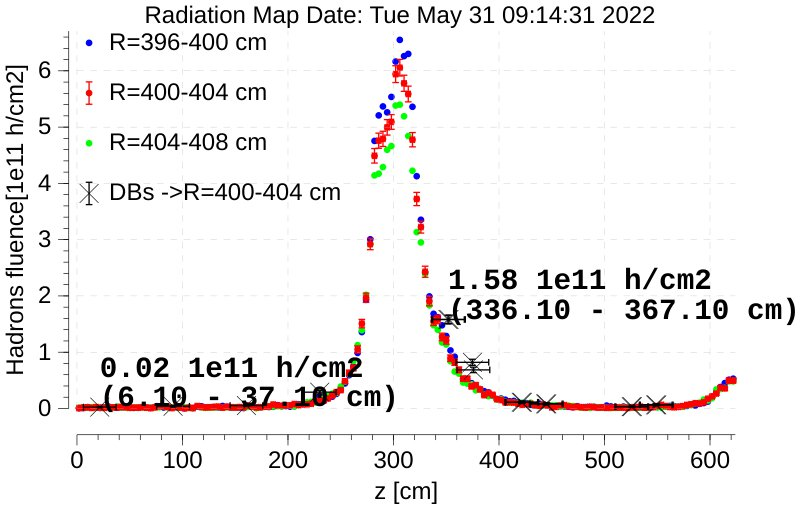
\includegraphics[width=0.8\linewidth]{assets/Eduardo_IEEE_NSS_MIC_RTSD_Poster-2_slide_1_item_8.jpeg}
\end{figure}

\begin{figure}[H]
\centering
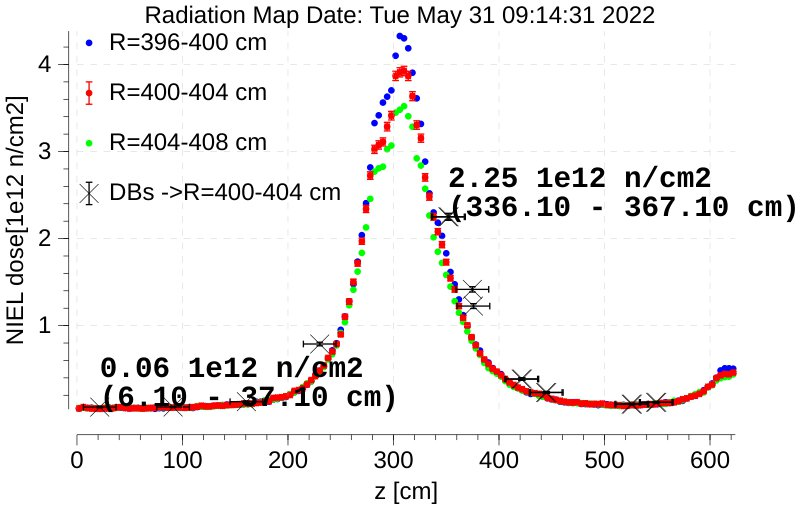
\includegraphics[width=0.8\linewidth]{assets/Eduardo_IEEE_NSS_MIC_RTSD_Poster-2_slide_1_item_9.jpeg}
\end{figure}

\begin{figure}[H]
\centering
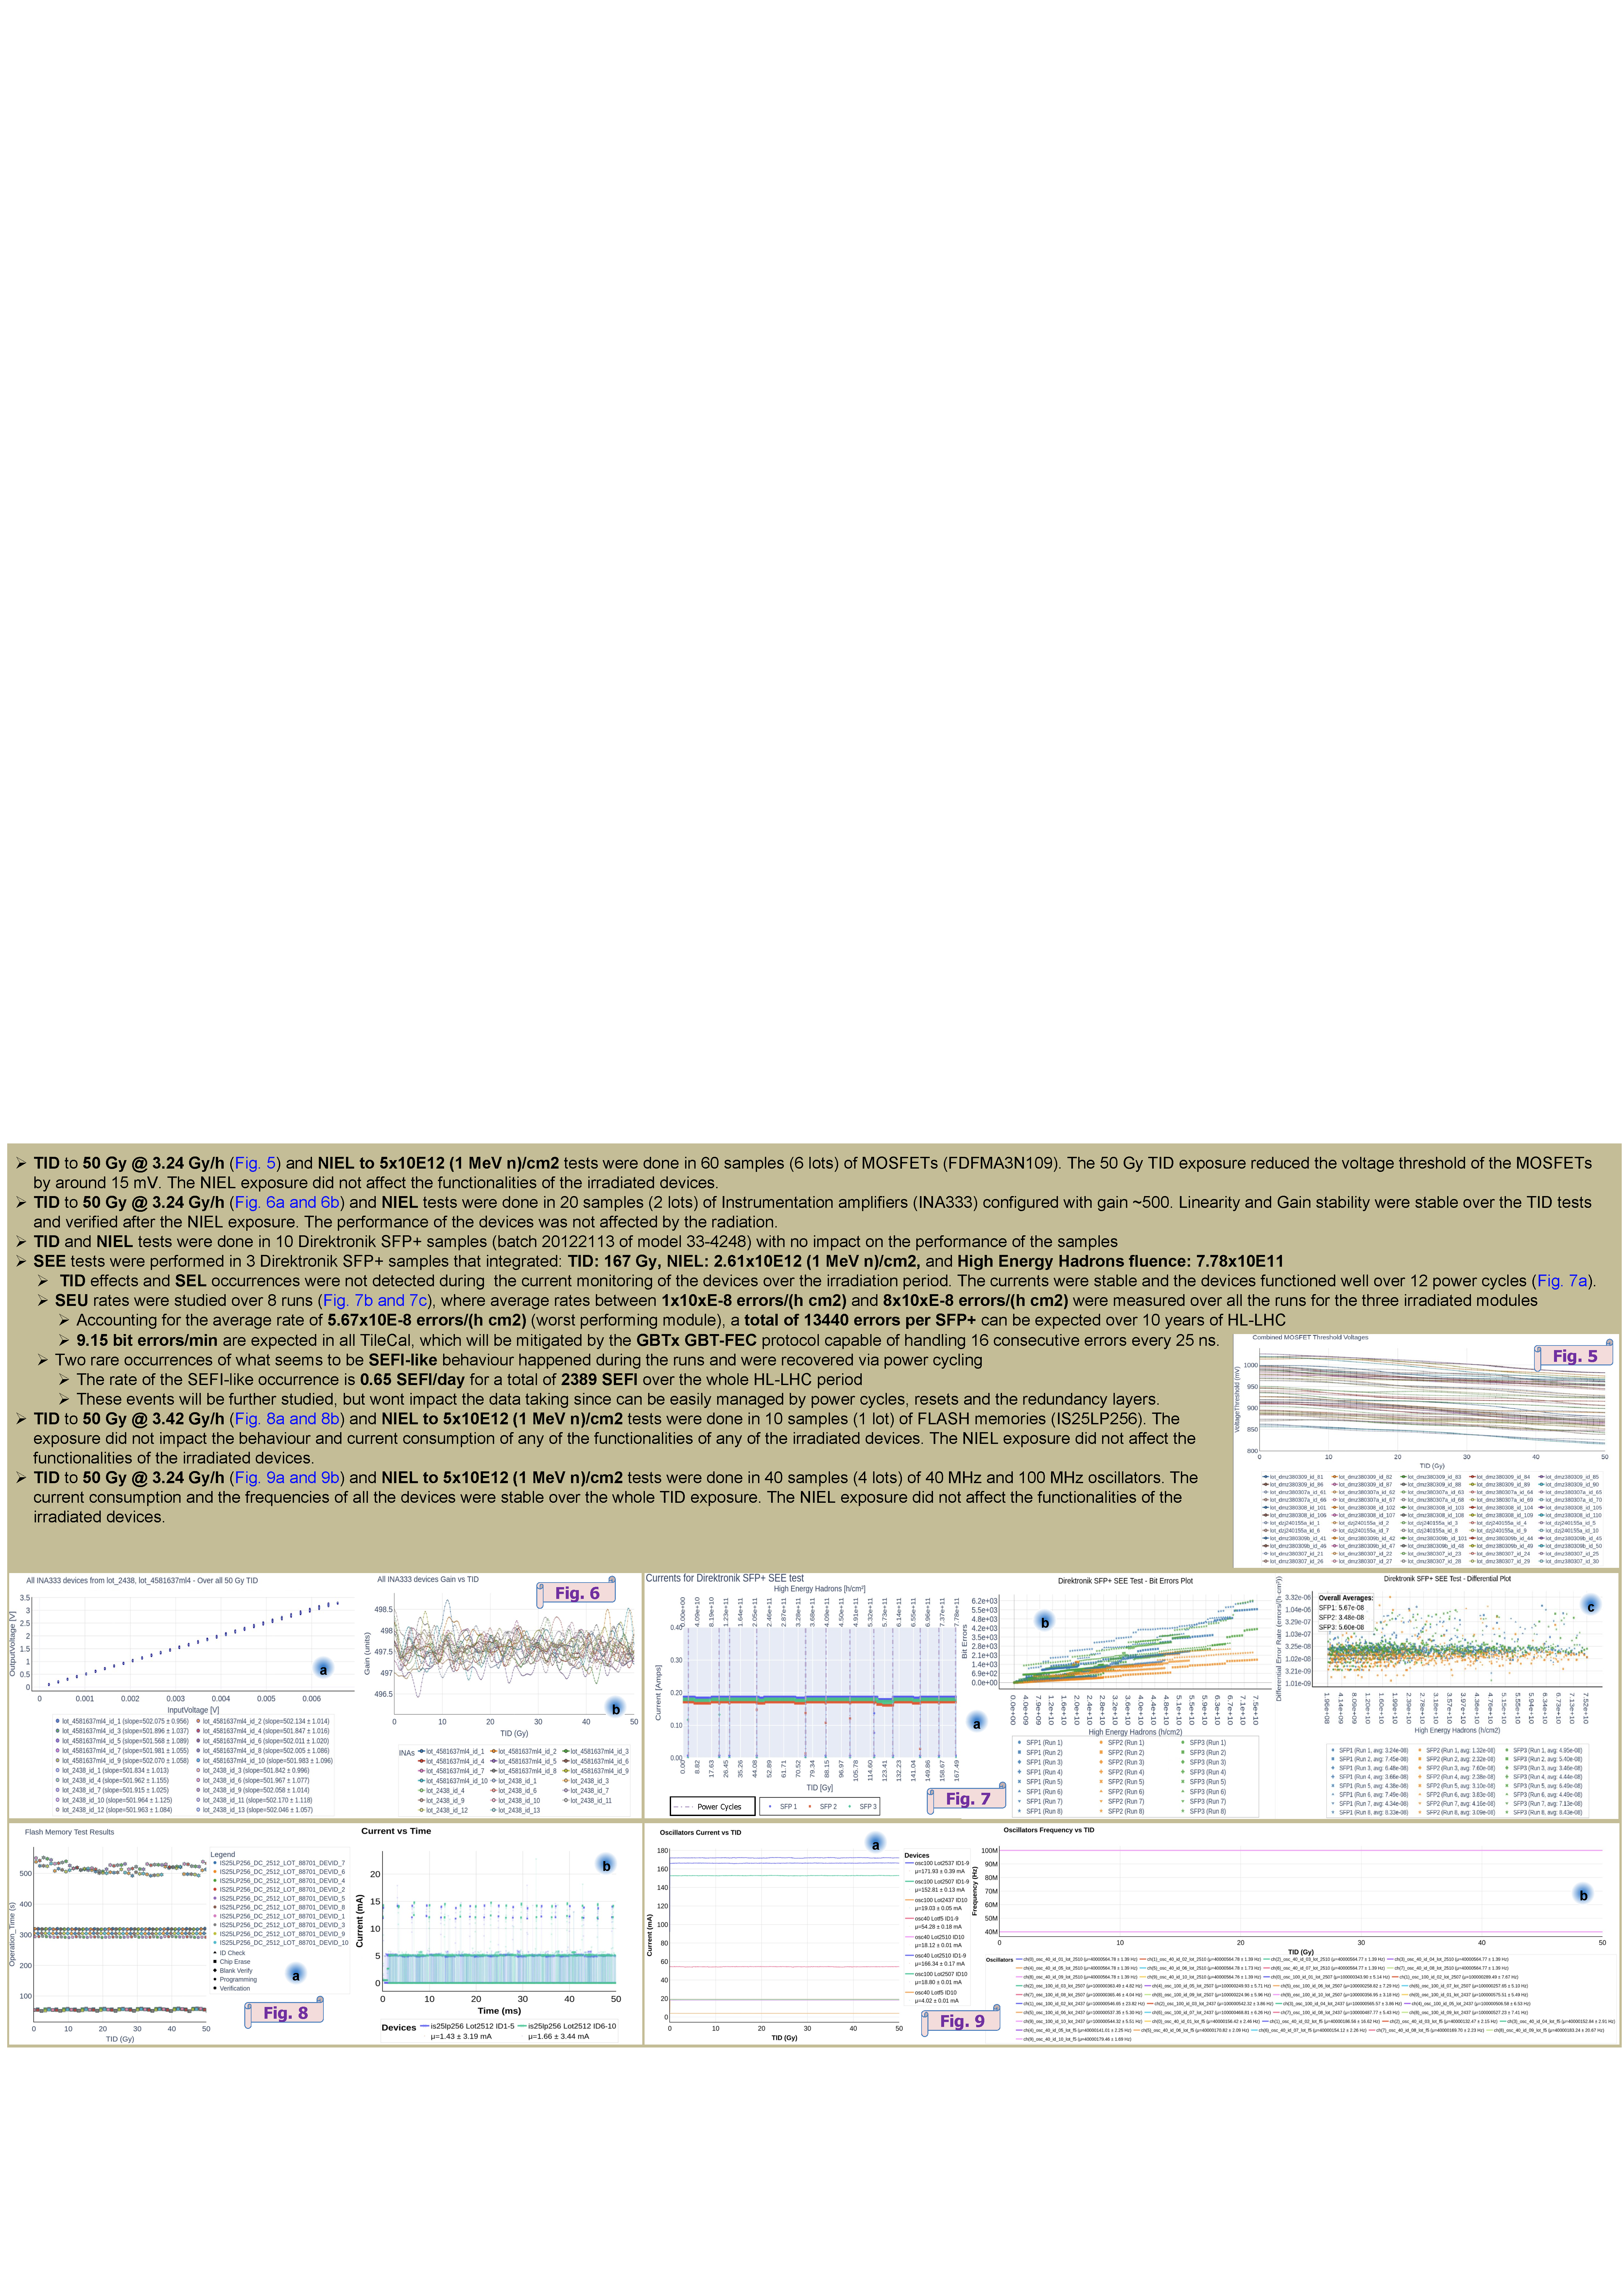
\includegraphics[width=0.8\linewidth]{assets/Eduardo_IEEE_NSS_MIC_RTSD_Poster-2_slide_1_item_10.pdf}
\end{figure}

\begin{figure}[H]
\centering
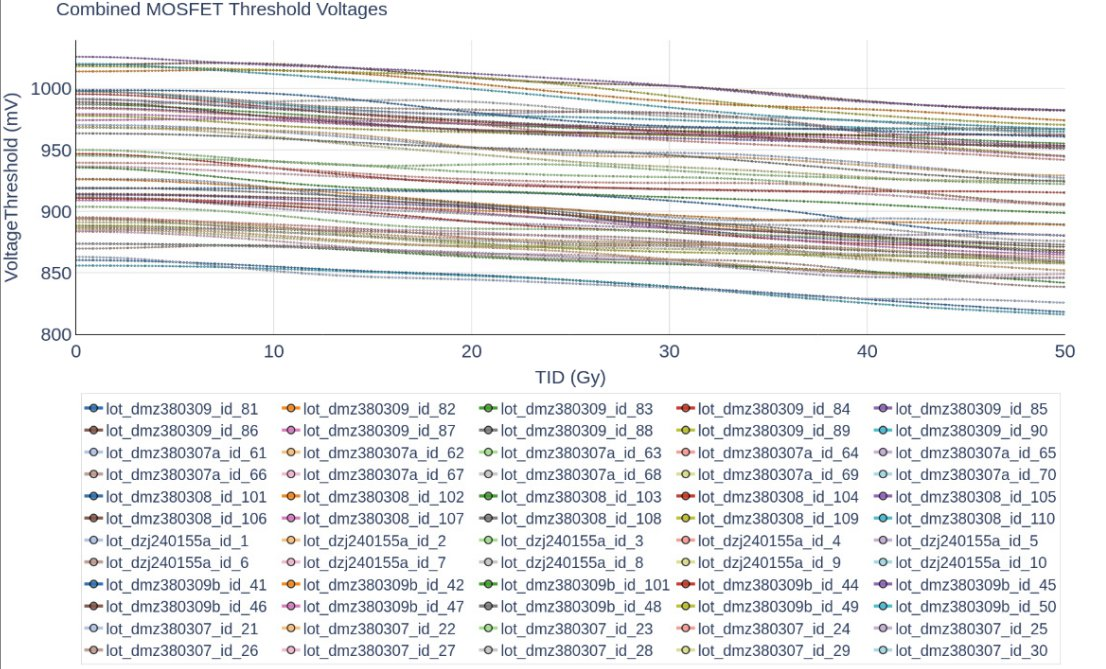
\includegraphics[width=0.8\linewidth]{assets/Eduardo_IEEE_NSS_MIC_RTSD_Poster-2_slide_1_item_11.jpeg}
\end{figure}

\begin{figure}[H]
\centering
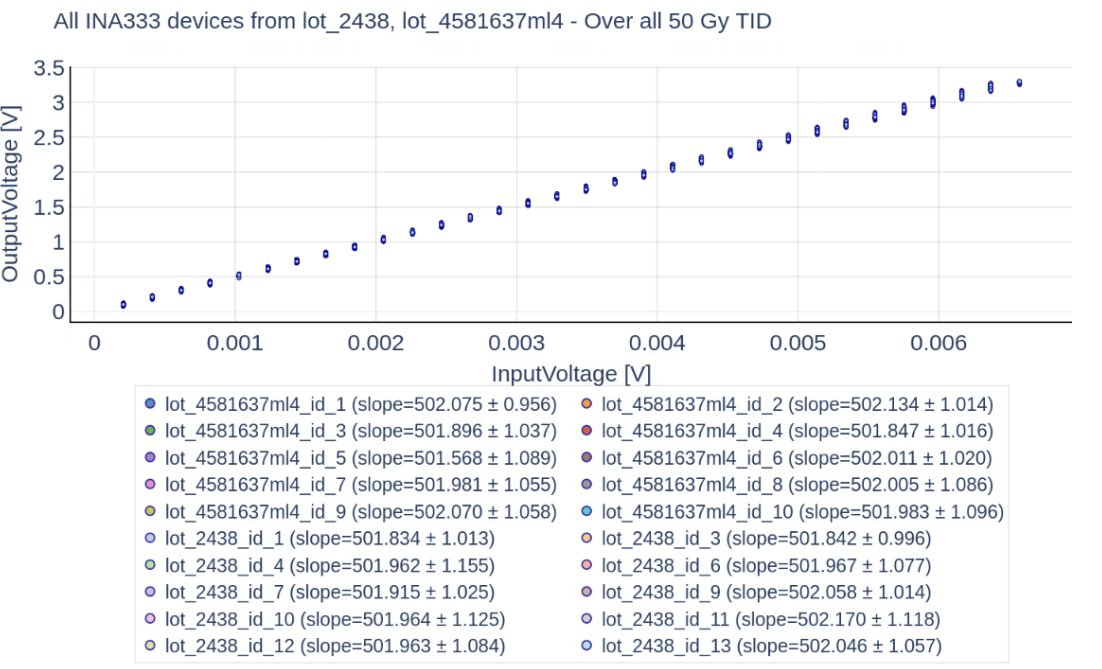
\includegraphics[width=0.8\linewidth]{assets/Eduardo_IEEE_NSS_MIC_RTSD_Poster-2_slide_1_item_12.jpeg}
\end{figure}

\begin{figure}[H]
\centering
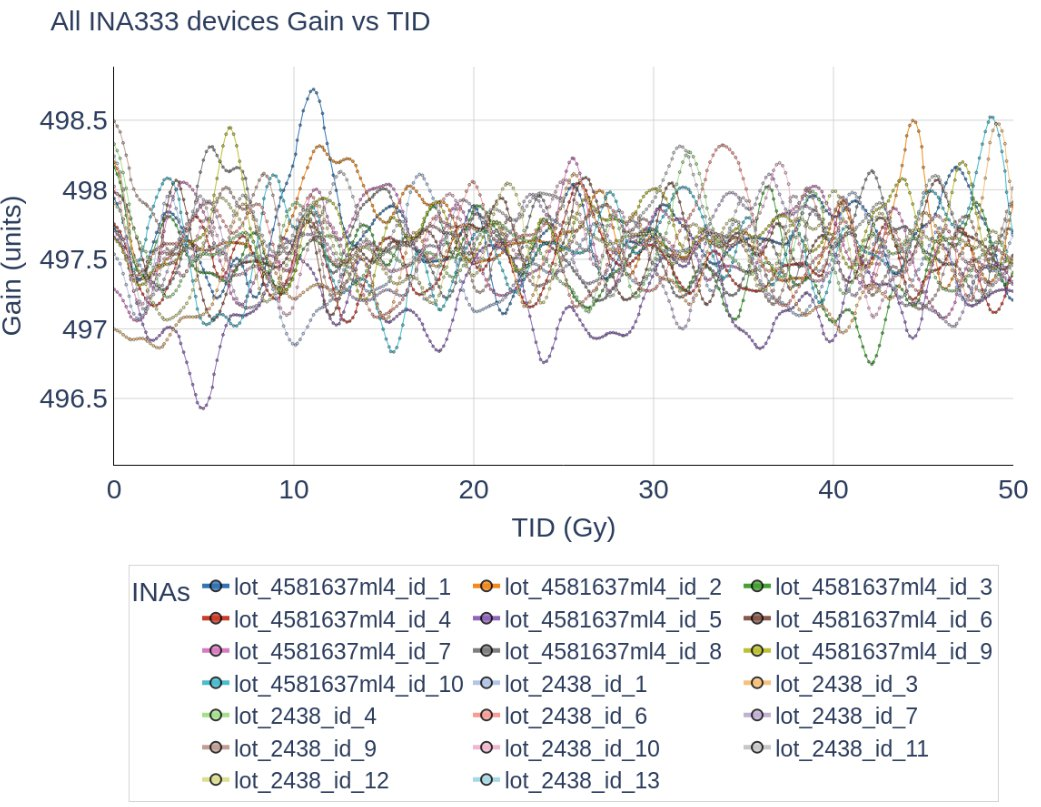
\includegraphics[width=0.8\linewidth]{assets/Eduardo_IEEE_NSS_MIC_RTSD_Poster-2_slide_1_item_13.jpeg}
\end{figure}

\begin{figure}[H]
\centering
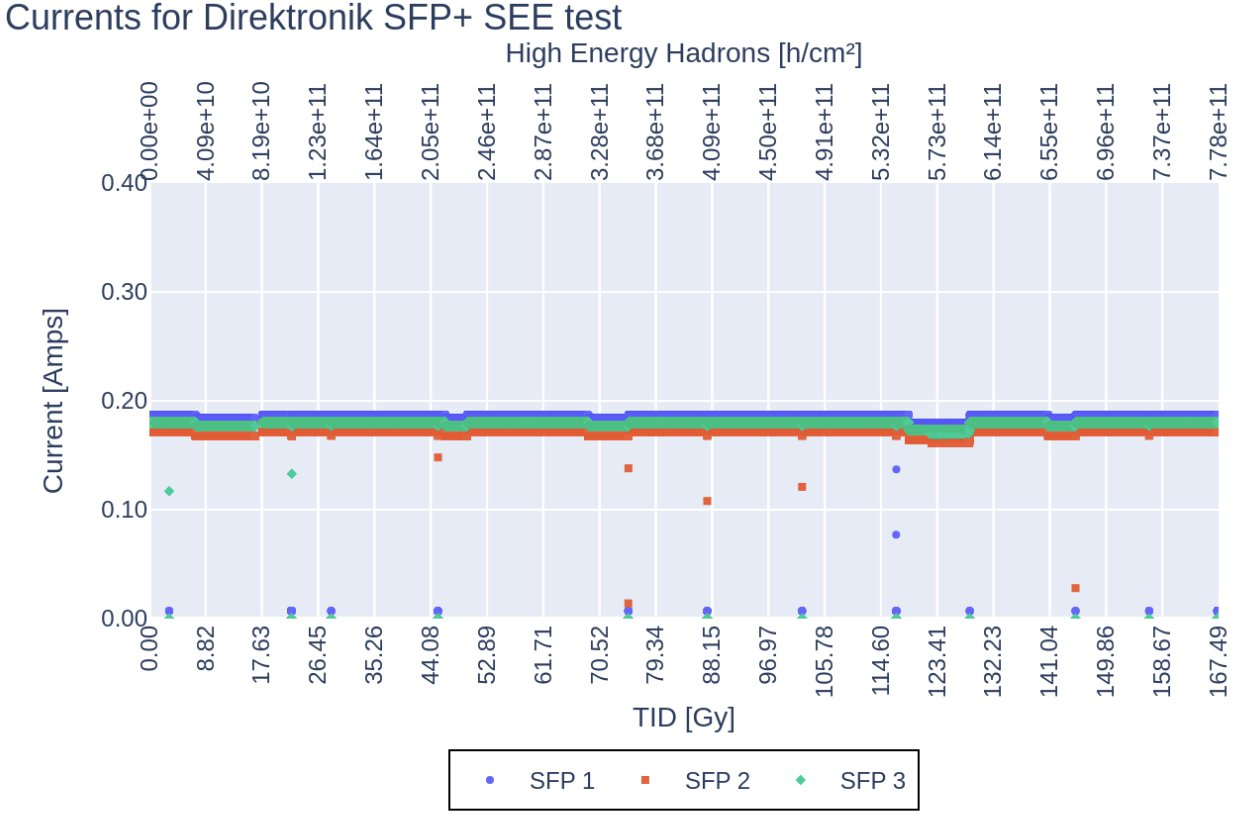
\includegraphics[width=0.8\linewidth]{assets/Eduardo_IEEE_NSS_MIC_RTSD_Poster-2_slide_1_item_14.jpeg}
\end{figure}

\begin{figure}[H]
\centering
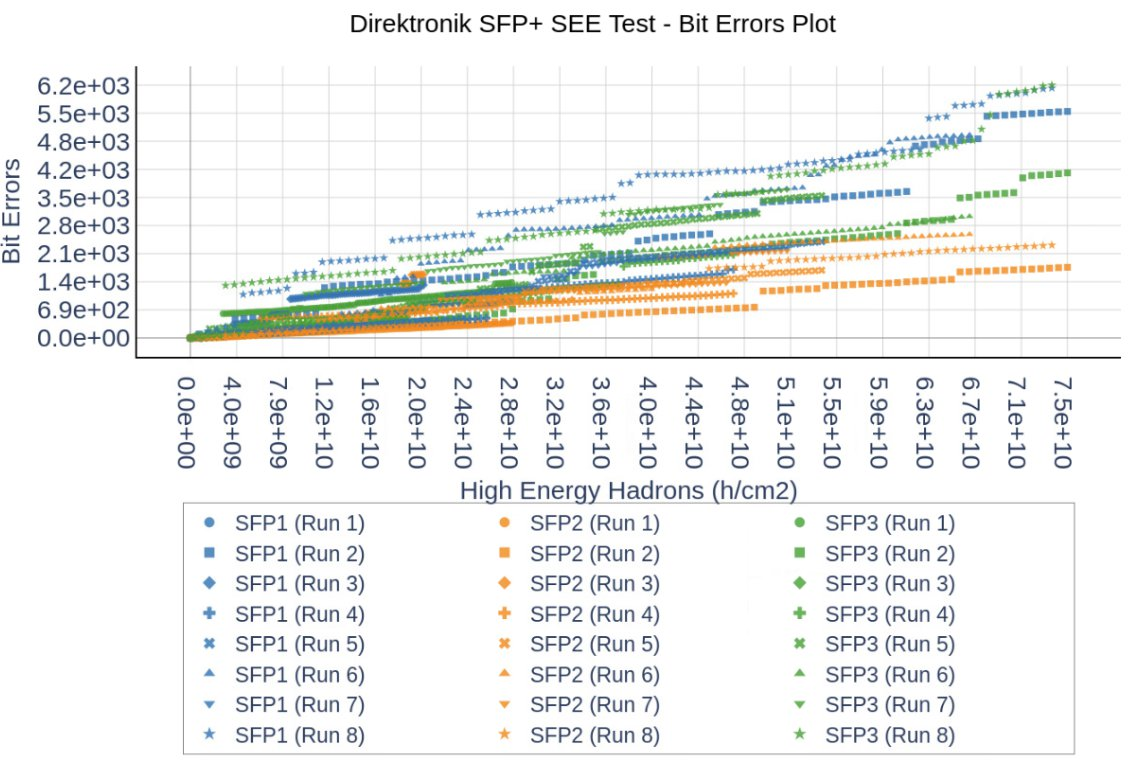
\includegraphics[width=0.8\linewidth]{assets/Eduardo_IEEE_NSS_MIC_RTSD_Poster-2_slide_1_item_15.jpeg}
\end{figure}

\begin{figure}[H]
\centering
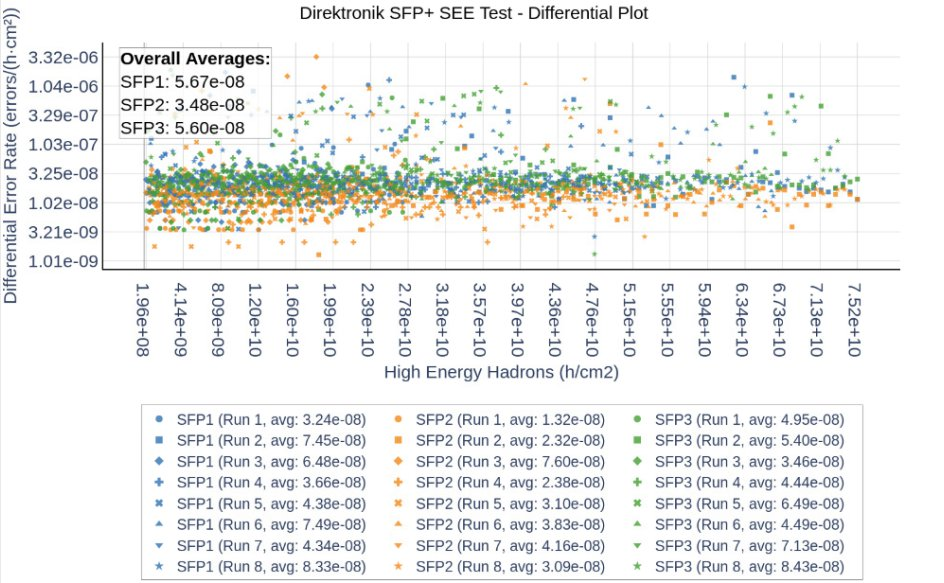
\includegraphics[width=0.8\linewidth]{assets/Eduardo_IEEE_NSS_MIC_RTSD_Poster-2_slide_1_item_16.jpeg}
\end{figure}

\begin{figure}[H]
\centering
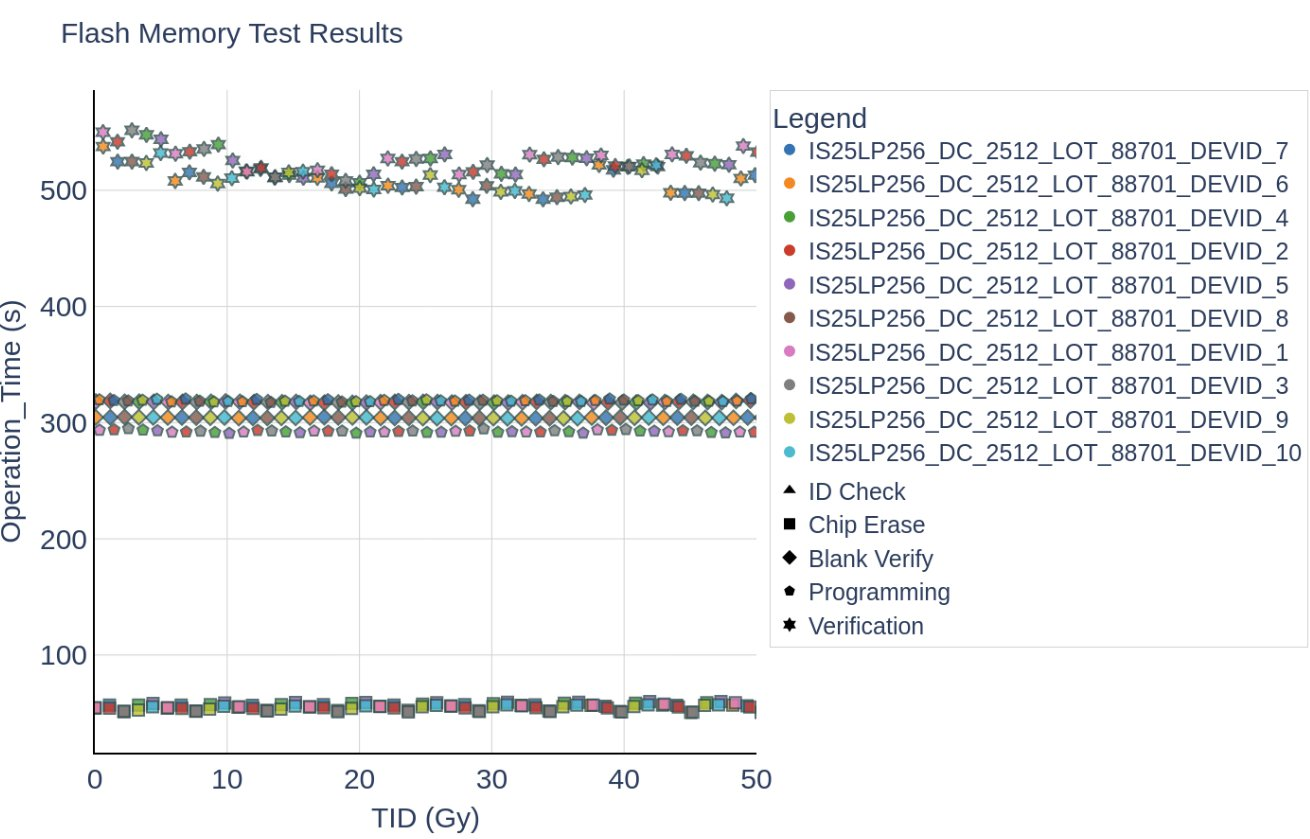
\includegraphics[width=0.8\linewidth]{assets/Eduardo_IEEE_NSS_MIC_RTSD_Poster-2_slide_1_item_17.jpeg}
\end{figure}

\begin{figure}[H]
\centering
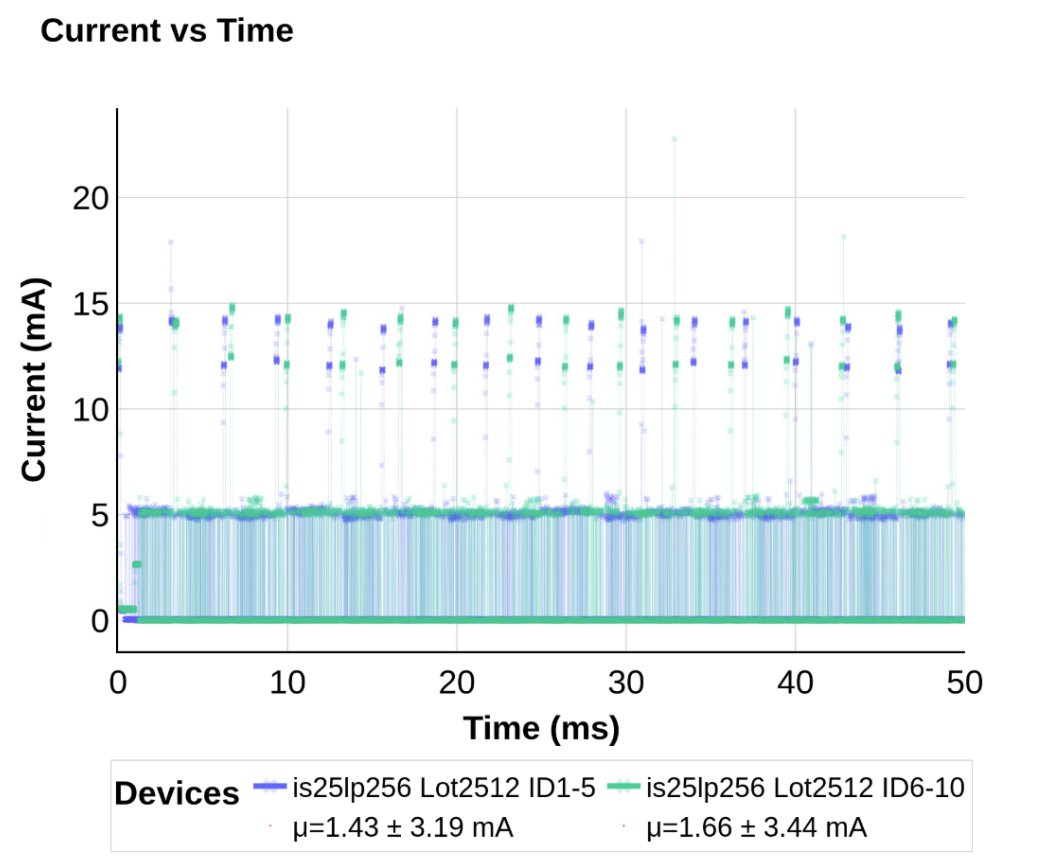
\includegraphics[width=0.8\linewidth]{assets/Eduardo_IEEE_NSS_MIC_RTSD_Poster-2_slide_1_item_18.jpeg}
\end{figure}

\begin{figure}[H]
\centering
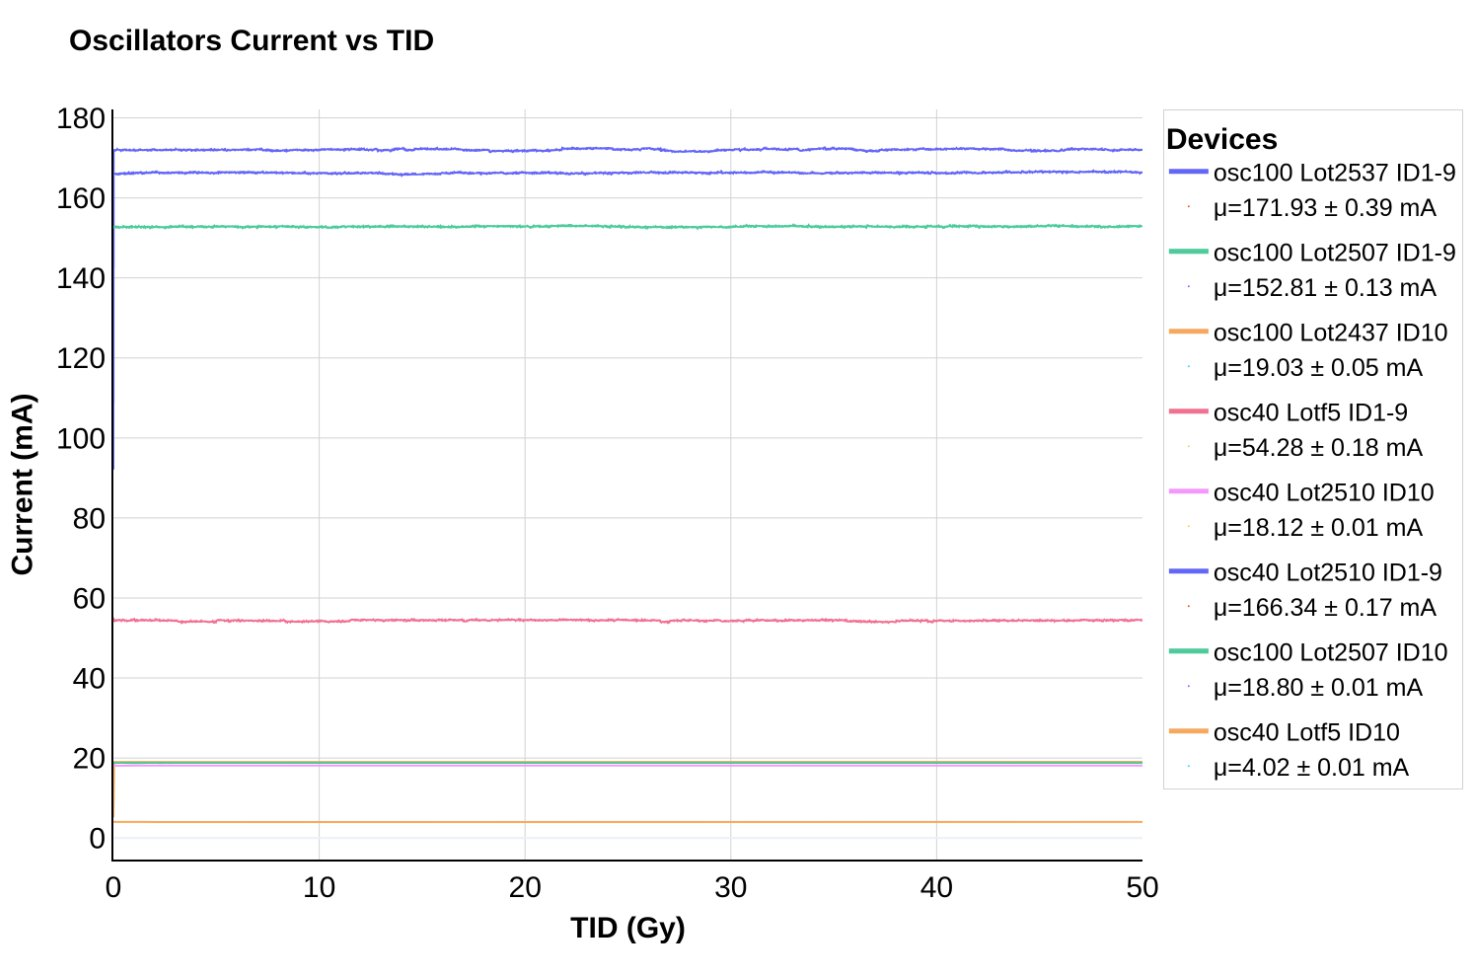
\includegraphics[width=0.8\linewidth]{assets/Eduardo_IEEE_NSS_MIC_RTSD_Poster-2_slide_1_item_19.jpeg}
\end{figure}

\begin{figure}[H]
\centering
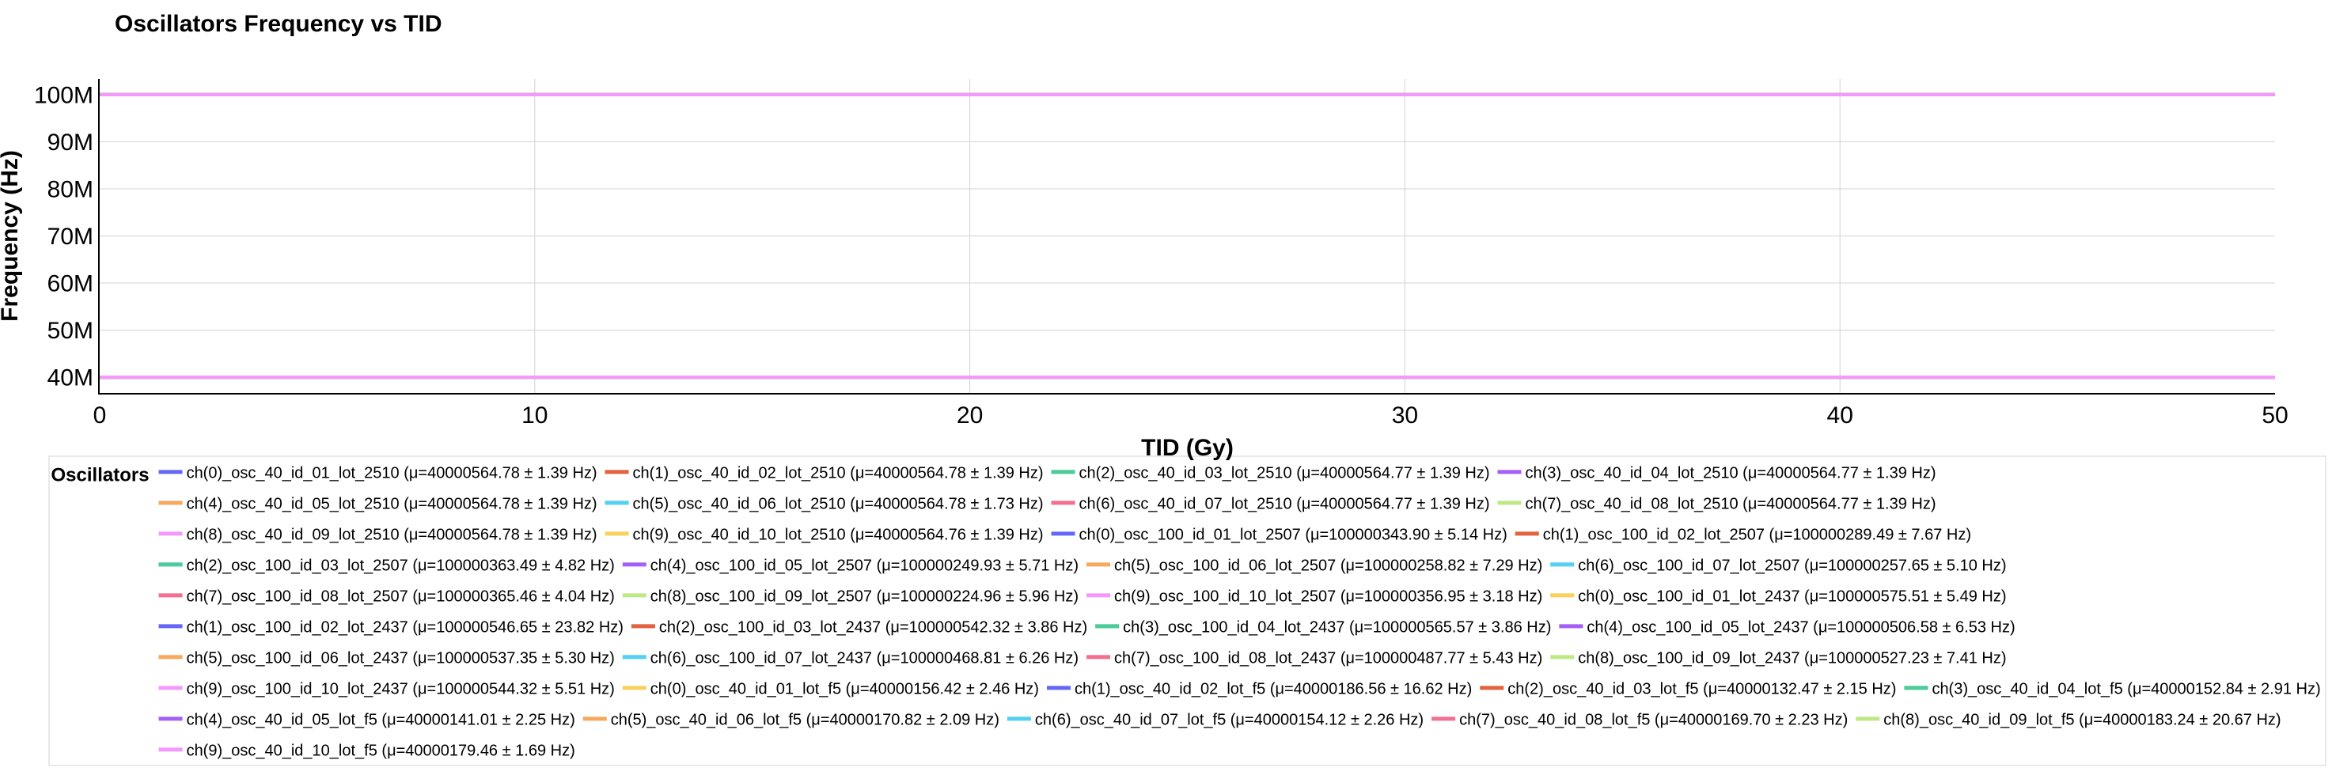
\includegraphics[width=0.8\linewidth]{assets/Eduardo_IEEE_NSS_MIC_RTSD_Poster-2_slide_1_item_20.jpeg}
\end{figure}

[1]   ATLAS   collaboration.   Technical   Design   Report   for   the   Phase-II   Upgrade   of   the   ATLAS   Tile   Calorimeter.   CERN- 
LHCC-   234   2017-019,   ATLAS-TDR-028,   2018 
[2]   ]   E.   Valdes   Santurio,   Development   of   the   read-out   link   and   control   board   for   the   ATLAS   Tile   Calorimeter 
Upgrade,   Ph.D.   Thesis,   Stockholm   University   (2019)   [ISBN:   978-91-7797-896-1] 
[3]   K.   Wyllie,   P.   Moreira   and   J.   Christiansen,   GBTX   MANUAL   V0.15   Technical   Report,   (2021), 
[4]   E.   Valdes,   Radiation   studies   performed   on   the   High   Luminosity   ATLAS   TileCal   link   Daughterboard,   DOI: 
10.1088/1748-0221/18/04/C04011 
[5]   E.   Valdes   ,   A   radiation   tolerant   read-out   link   and   control   Daughterboard   for   the   upgrade   the   of   the   ATLAS 
Hadronic   Calorimeter,   ATL-TILECAL-SLIDE-2023-619,   https://cds.cern.ch/record/2880342/files/ATL-TILECAL-SLIDE- 
2023-619.pdf

The component selection tested for the production of the ATLAS TileCal DB fulfill the HL-LHC radiation requirements following the current collaboration guidelines and 
simulations for TID, NIEL and SEE. Most of the components have been acquired and qualified in radiation on a lot basis for pre-production and production phases. 
Radiation campaigns to test the DC-DC converters (LTM4691), ProASIC and KU FPGA acquired lots will take place during end 2025 and 2026. Around 930 DBs will 
be produced during 2026 and 2027 as the contribution of Stockholm University to the HL-LHC era for TileCal.

Eduardo Valdes Santurio 
Researcher at Fysikum, Stockholm University. Email:  eduardo.valdes@fysik.su.se ,  eduardo.valdes@cern.ch 
Co-authors: Samuel Silverstein, Christophe Clement, Christian Bohm, Riccardo Vari, Massimo Corradi, Federico Morodei and Sabrina Perrella.

\end{document}
